\chapter{Version Control with Git}
\section{Version Control System}
Version control systems (VCS) are tools designed to help manage changes to documents, code, and other complex projects over time. This is particularly important in projects where multiple collaborators are working simultaneously on the same files, ensuring consistency and traceability. In the absence of such systems, keeping track of different versions often leads to confusion and disorganization, where it becomes difficult to track which version is current or accurate.

The need for version control becomes critical in scenarios such as:
\begin{itemize}
    \item \textit{Complex Projects:} Documents or codebases that evolve over time require systematic tracking of changes.
    \item \textit{Collaboration:} Multiple developers or team members often work on the same files, potentially introducing conflicting changes.
    \item \textit{Parallel Versions:} Projects may have multiple branches for testing, development, and stable releases running concurrently.
    \item \textit{Reproducibility:} For debugging or tracking down issues, it’s crucial to revert to earlier versions and understand the evolution of the project.
\end{itemize}

A VCS offers several vital features:
\begin{enumerate}
    \item \textit{Consistent Labeling:} Each revision is labeled consistently to allow for easy identification of different versions.
    \item \textit{Tracking Changes:} Differences between revisions are logged, ensuring a clear history of modifications.
    \item \textit{Metadata:} Information such as dates, authors, and commit messages are associated with each change.
    \item \textit{Revisions:} The ability to create point-in-time snapshots of the entire project is critical for ensuring consistency.
    \item \textit{Collaboration:} Multiple developers can work on the same codebase concurrently, with features such as branching and merging to avoid conflicts.
\end{enumerate}

There are three primary types of VCS:
\begin{enumerate}
    \item \textit{Local Version Control System:} A local VCS stores changes on the user's computer. Although it provides basic version tracking, collaboration is difficult without additional tools (see Figure \ref{fig:lvcs}).

    \begin{figure}[ht]
        \centering
        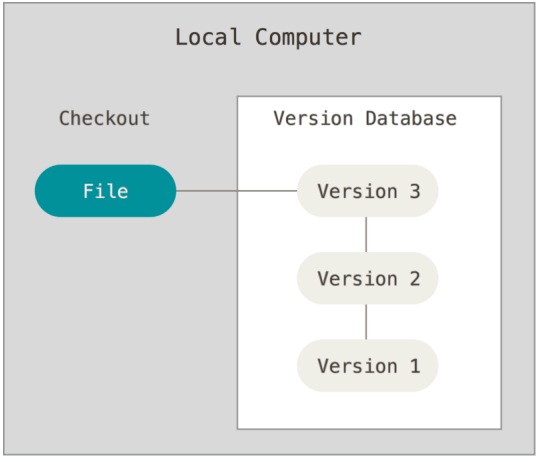
\includegraphics[width=7cm]{images/lvcs.PNG}
        \caption{Local Version Control System}
        \label{fig:lvcs}
    \end{figure}
    
    \item \textit{Centralized Version Control System (CVCS):} Centralized systems, use a single central server to store all versions of a project. Developers check out a working copy from the central repository, make changes, and commit them back (see Figure \ref{fig:cvcs}).

    \begin{figure}[ht]
        \centering
        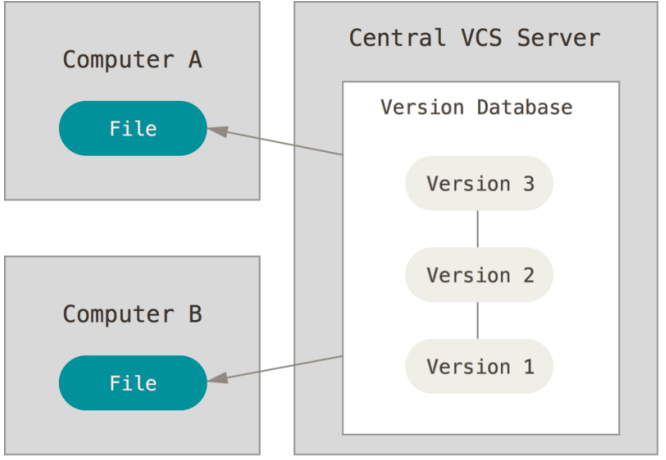
\includegraphics[width=9cm]{images/cvcs.PNG}
        \caption{Centralized Version Control System}
        \label{fig:cvcs}
    \end{figure}
    
    \item \textit{Distributed Version Control System (DVCS):} In DVCS, such as Git and Mercurial, each user has a full copy of the repository, including its history. This allows for full collaboration even without a central server, with users able to synchronize changes between repositories (see Figure \ref{fig:dvcs}).

    \begin{figure}[ht]
        \centering
        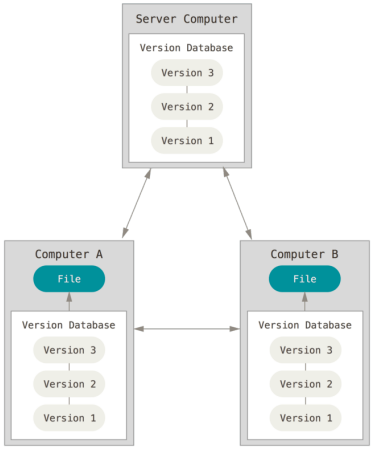
\includegraphics[width=9cm]{images/dvcs.PNG}
        \caption{Distributed Version Control System}
        \label{fig:dvcs}
    \end{figure}
\end{enumerate}


Key Version Control Terminology
Understanding some basic VCS terms is essential for working with any system:

Working Copy: The project files on your local machine that are tracked by the VCS.
Commit: A snapshot of the repository at a specific point in time. Commits include changes, metadata (author, date), and often a commit message explaining the changes.
Branch: A separate line of development. Branches allow for parallel work without affecting the main project. Each branch is essentially a sequence of commits.
Merge: The process of combining changes from one or more branches into another. Merging helps integrate parallel work.
Tag: A custom label applied to a specific commit. Tags are used to mark important milestones such as releases.
Repository: The complete set of commits, branches, and tags for a project. It represents the entire history of changes made to the project.
Fork: A personal copy of someone else's repository, typically used for developing independent changes that can later be merged back.
Pull/Merge Request: A request to merge changes from one branch or fork into another, typically used in collaborative development workflows.

\section{Git}
Git is a distributed version control system (DVCS) created by Linus Torvalds in 2005 to manage the Linux kernel’s source code. Git is designed to efficiently handle everything from small to very large projects with speed and flexibility. It uses concepts like Directed Acyclic Graphs (DAG) and Merkle Trees for data integrity and fast operation.

\subsection*{Git Commit}
A commit is a snapshot of the project at a given moment. It can include any subset of files, and each commit has one or more parent commits, except for the very first commit (which is an orphan). Commits require a meaningful message to explain the changes (see Table \ref{tab:commit_structure}).

\begin{table}[h]
    \centering
    \begin{tabular}{|l|p{10cm}|}
    \hline
    \textbf{Component}           & \textbf{Description}                                                                \\ \hline
    Commit message               & A short description of the changes made.                                             \\ \hline
    Committer and date           & The person who made the commit and when it was committed.                            \\ \hline
    Author and author date       & The original author of the change.
                 \\ \hline
    Tree                         & A hash representing all files in the commit.                                         \\ \hline
    Parent commits               & One or more references to previous commits.                                          \\ \hline
    Commit ID                    & A SHA-1 hash of the commit's content.                                                \\ \hline
    \end{tabular}
    \caption{Structure of a Commit}
    \label{tab:commit_structure}
\end{table}

\subsection*{Git Staging Area}
The staging area is where files are added before committing. Only files in the staging area will be included in the next commit. This allows the developer to carefully curate changes to be committed.

\subsection*{Branching in Git}
A branch is a line of development, essentially a sequence of commits. Branches allow for parallel development, such as creating a new feature or testing code without affecting the main project. When a branch is ready to be incorporated back into the main project, a merge occurs.

The main branch (often called main or master) is the default branch where final code lives. Branches can be merged back into the main branch after development is completed.

\begin{Example}{Branching in Git}{}
In this diagram, we see two branches of development in a Git repository: the \texttt{master} branch and a feature branch called \texttt{test-new-algorithm}.

\begin{minipage}{\textwidth}
    \centering
    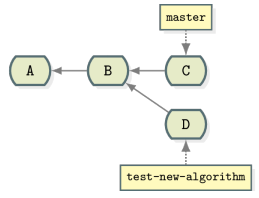
\includegraphics[width=0.4\textwidth]{images/es-branch-git.PNG}
    %\captionof{figure}{Esempio}
\end{minipage}
    
Commit C is part of the master branch. This means that after commit B, a commit was made to the master branch. Commit D is part of the feature branch called \texttt{test-new-algorithm}, which diverged from commit B. This means that after commit B, a new branch was created to work on a different feature or experiment, which resulted in commit D. 

Eventually, these two branches (the master and feature branch) might need to be merged. The goal of merging would be to integrate the changes made in both the branches.
\end{Example}

\subsection*{The HEAD}
HEAD is a pointer to the current branch or commit you are working on. The files in your working directory reflect the state of the commit that HEAD points to. When HEAD points directly to a commit instead of a branch, it is referred to as a detached HEAD, which prevents committing new changes until you reattach it to a branch.

\subsection*{Tags in Git}
Tags are labels used to mark specific commits, often for significant events like software releases. Tags help quickly find important points in a project's history. Although tags can be removed, it’s generally best practice to avoid doing so.

\subsection*{Merge Strategies}
When merging branches, there are different strategies:
\begin{enumerate}
    \item \textit{Fast-forward merge:} Occurs when the branch being merged has no new commits since it branched off. The branch simply advances to include the new commits.
    \item \textit{Non-fast-forward merge:} Used when the two branches have diverged, requiring a merge commit to reconcile differences.
    \item \textit{Rebase:} An alternative to merging that replays commits from one branch onto another, resulting in a cleaner project history without merge commits.
\end{enumerate}

\begin{Example}{Fast-Forward Merge in Git}{}
The \texttt{master} branch is currently pointing to commit C, while the experimental branch has advanced and contains commits E and F.

\begin{minipage}{\textwidth}
    \centering
    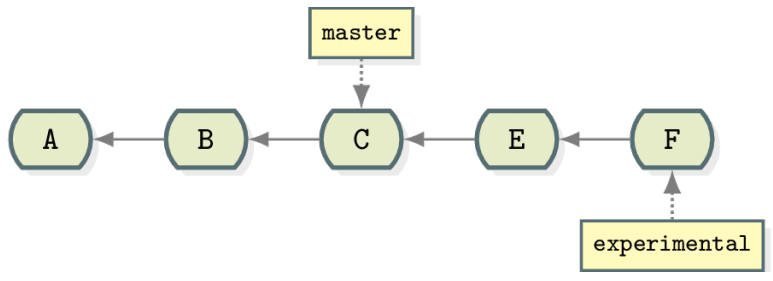
\includegraphics[width=0.6\textwidth]{images/fast-forward-merge.PNG}
    %\captionof{figure}{Esempio}
\end{minipage}

After performing a fast-forward merge, the \texttt{master} branch now points to commit F, which was the latest commit in the \texttt{experimental} branch. No new merge commit is created because fast-forward simply moves the pointer of the \texttt{master} branch to the latest commit of the merged branch (in this case, commit F). The history appears linear, as if the \texttt{experimental} changes were part of the original development line all along.
\end{Example}

\begin{Example}{Non-Fast-Forward Merge in Git}{}
In the first diagram, we observe two branches: \texttt{master} is pointing to commit E and \texttt{experimental} is pointing to commit F, which diverged from the \texttt{master} branch at commit C.

\begin{minipage}{\textwidth}
    \centering
    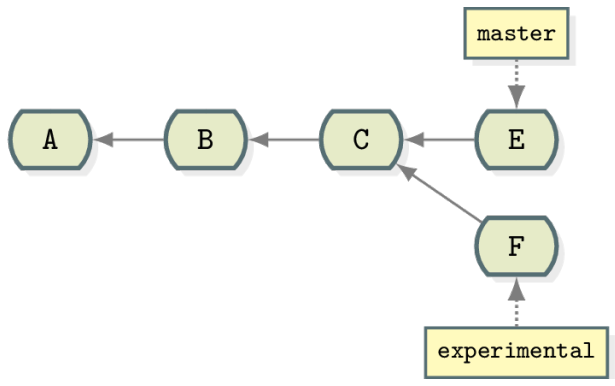
\includegraphics[width=0.5\textwidth]{images/non-fast-forward-merge1.PNG}
    %\captionof{figure}{Esempio}
\end{minipage}

After the merge, a non-fast-forward merge is performed, and a new commit G is created, which contains the merged changes from both the \texttt{master} and \texttt{experimental} branches. The \texttt{master} branch is now updated to point to this new merge commit G. The \texttt{experimental} branch remains unchanged and still points to commit F.

\begin{minipage}{\textwidth}
    \centering
    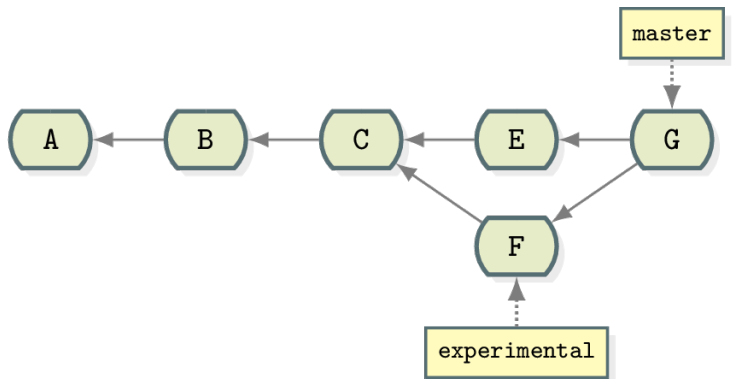
\includegraphics[width=0.5\textwidth]{images/non-fast-forward-merge.PNG}
    %\captionof{figure}{Esempio}
\end{minipage}
\end{Example}

\begin{Example}{Rebase Merge in Git}{}
We see two branches: \texttt{master} is pointing to commit D and \texttt{experimental} has diverged from the master at commit B and points to commit F, with commit E as an intermediate step.

\begin{minipage}{\textwidth}
    \centering
    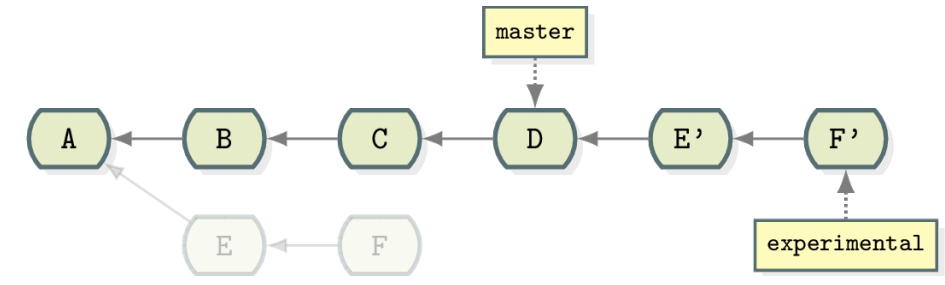
\includegraphics[width=0.6\textwidth]{images/rebase-merge.PNG}
    %\captionof{figure}{Esempio}
\end{minipage}

After the rebase, the \texttt{experimental} branch has been rebased onto the \texttt{master} branch: the commits E and F have been rewritten as new commits E' and F'. The \texttt{experimental} branch now appears as if it was developed directly on top of commit D (the latest commit on the \texttt{master} branch). The old commits E and F are no longer referenced in the new history, effectively making them obsolete. It replays the changes from \texttt{experimental} on top of the \texttt{master} branch, ensuring that the history appears linear and avoids a merge conflict.
\end{Example}

\subsection*{Merge Conflict}
Merge conflicts arise when we merge branches, using non-fast-forward or rebase strategies, that modify the same part of a file in incompatible ways. Git will alert you to the conflict, and you must manually resolve it by choosing one of the following:
\begin{itemize}
    \item \textit{Edit the file manually:} Combine the changes as needed.
    \item \textit{Keep "ours":} Use your version of the file.
    \item \textit{Keep "theirs":} Use the other branch’s version.
\end{itemize}

\subsection*{Remote Git Repositories}
Git allows users to interact with remote repositories, which are hosted on remote servers. These repositories can store and share commits, branches, and tags. The most common remote repository is called origin, which is typically set as the default when a repository is cloned from a URL. A common workflow involves:
\begin{itemize}
    \item \textit{Cloning:} Cloning creates a local copy of a remote Git repository using a URL. This process downloads all the commits, branches, and tags into the local system. The remote URL from which the repository is cloned is assigned as the origin remote.
    \item Pushing: Once changes are committed locally, they can be sent to the remote repository using the \texttt{push} command. This uploads the local commits, branches, and tags to the remote.
    \item Fetching and Pulling: Fetch retrieves the latest changes from the remote repository, including commits, branches, and tags, but does not automatically merge them into your local branches. Pull is a combination of fetch and merge. After fetching the latest changes from the remote, Git automatically merges them into the current branch.
\end{itemize}

\begin{Example}{Git clone}{}
\begin{wrapfigure}{r}{0.25\textwidth}
    \vspace{-0.5cm}
    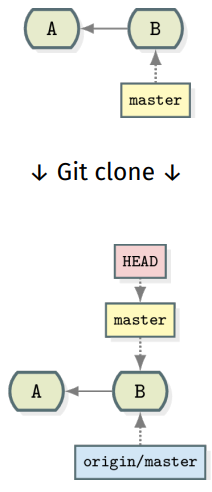
\includegraphics[width=0.20\textwidth]{images/git-clone.PNG}
    \vspace{-0.5cm}
\end{wrapfigure}

The diagram illustrates two states: the remote repository and the local repository after cloning. At the top, the remote repository is represented with two commits: Commit \texttt{A} and Commit \texttt{B}. The \texttt{master} branch pointer is positioned at commit \texttt{B}, indicating that this is the latest commit on the \texttt{main} branch.

Once the cloning operation is complete, we observe the local setup: The commits \texttt{A} and \texttt{B} are copied to the local repository. A local branch named \texttt{master} is created, pointing to commit \texttt{B}, similar to the remote. The HEAD points to the local \texttt{master} branch. The local repository also tracks the remote branch with the pointer \texttt{origin/master}, which is a reference to the latest commit on the remote repository’s \texttt{master} branch. This tracking allows the local repository to know where the remote branch is in relation to the local copy.

\vspace{.8cm}
\end{Example}

\begin{Example}{Git push}{}
Before the push, the remote repository initially has two commits: \texttt{A} and \texttt{B} and the \texttt{master} branch pointer is positioned at commit \texttt{B}, indicating that it is the latest commit in the repository. The local repository contains the same two commits as the remote repository.

\begin{minipage}{\textwidth}
    \centering
    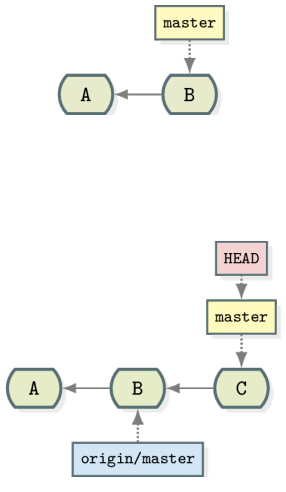
\includegraphics[height=0.5\textwidth]{images/git-push1.PNG}
    \hspace{1cm}
    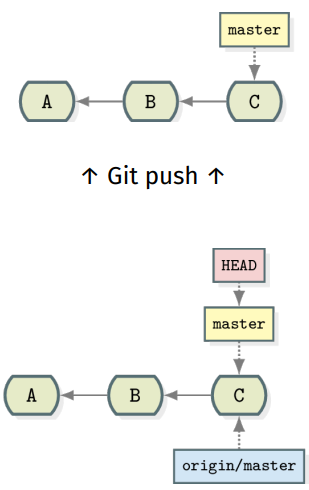
\includegraphics[height=0.5\textwidth]{images/git-push2.PNG}
    %\captionof{figure}{Esempio}
\end{minipage}
    
A new commit, \texttt{C}, has been made in the local repository, but it has not yet been pushed to the remote. The HEAD is pointing to the local \texttt{master} branch, which now includes commit \texttt{C}. The \texttt{origin/master} pointer still points to commit \texttt{B}, because that is where the remote repository is.
    
The \texttt{Git push} command sends the new commit from the local repository to the remote repository. This action updates the remote repository with the local changes. After the push, the remote repository now contains commit \texttt{C} in addition to \texttt{A} and \texttt{B}. The \texttt{master} branch in the remote repository is updated to point to commit \texttt{C}, reflecting the new changes pushed from the local repository. The local repository remains the same after the push, with the HEAD still pointing to commit \texttt{C}. The \texttt{origin/master} reference is updated to commit \texttt{C}, indicating that the local and remote repositories are now synchronized, both containing commits \texttt{A}, \texttt{B}, and \texttt{C}.
\end{Example}

\begin{Example}{Git fetch}{}
\begin{minipage}{\textwidth}
    \centering
    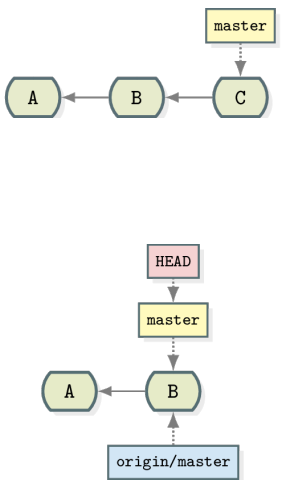
\includegraphics[height=0.5\textwidth]{images/git-fetch1.PNG}
    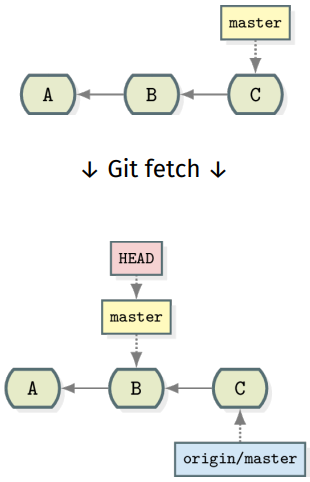
\includegraphics[height=0.5\textwidth]{images/git-fetch2.PNG}
    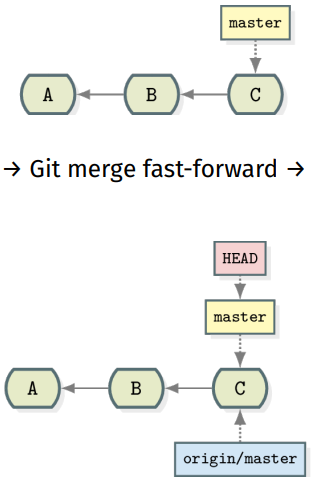
\includegraphics[height=0.5\textwidth]{images/git-fetch3.PNG}
    %\captionof{figure}{Esempio}
\end{minipage}

Before the fetch, the remote repository has commits \texttt{A}, \texttt{B}, and \texttt{C} on the \texttt{master} branch and the local repository only has commits \texttt{A} and \texttt{B}, and the \texttt{master} branch points to \texttt{B}. There's also an outdated reference to the remote branch, \texttt{origin/master}, still pointing to commit \texttt{B}. At this point, the local repository is not up to date with the latest commit (\texttt{C}) from the remote \texttt{master} branch.

After running \texttt{git fetch}, the local repository retrieves the latest state of the remote branch. No changes have occurred in the remote repository; it still has commits \texttt{A}, \texttt{B}, and \texttt{C} on the \texttt{master} branch. The local \texttt{origin/master} reference is updated to point to commit \texttt{C}, reflecting the state of the remote repository. However, the local \texttt{master} branch still points to \texttt{B}, indicating that the local working branch has not yet been merged with the new changes. At this stage, the local repository has retrieved the latest remote changes, but they have not been integrated into the local branch (\texttt{master}).

After running a fast-forward merge (\texttt{git merge --ff-only}), the local branch is updated. Again, no changes in the remote repository. The local \texttt{master} branch is now updated to commit \texttt{C}, aligning with \texttt{origin/master}. This is a fast-forward merge because the local branch was directly behind the remote branch, with no new changes of its own. As a result, the \texttt{master} branch simply advances forward to the latest commit (\texttt{C}) without creating any merge commit.
\end{Example}

\begin{Example}{Git pull}{}
Before git pull, the remote \texttt{master} branch has commits \texttt{A}, \texttt{B}, and \texttt{C} and the local repository is behind the remote and only has commits \texttt{A} and \texttt{B}. The HEAD and \texttt{master} branch in the local repository point to commit \texttt{B}, while the remote-tracking branch (\texttt{origin/master}) also points to \texttt{B}. This means the local repository hasn't fetched or pulled the latest changes from the remote, which includes commit \texttt{C}. At this point, the local branch needs to be updated to include the changes made in the remote repository.

\begin{minipage}{\textwidth}
    \centering
    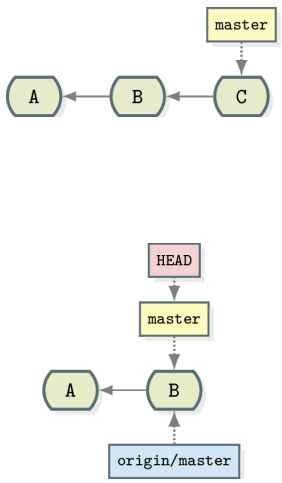
\includegraphics[height=0.5\textwidth]{images/git-pull1.PNG}
    \hspace{1cm}
    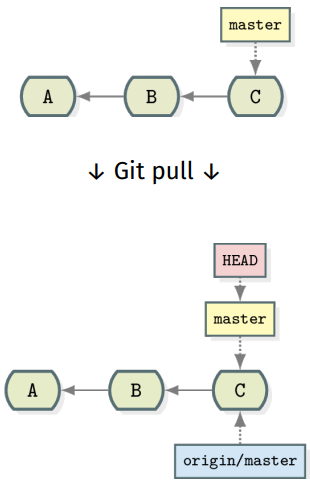
\includegraphics[height=0.5\textwidth]{images/git-pull2.PNG}
    %\captionof{figure}{Esempio}
\end{minipage}

After running \texttt{git pull}, no changes occur in the remote repository, which still has commits \texttt{A}, \texttt{B}, and \texttt{C} on the \texttt{master} branch. The local repository now has commit \texttt{C} after the \texttt{pull} operation. Both the \texttt{master} branch and the remote-tracking branch (\texttt{origin/master}) point to commit \texttt{C}, and the HEAD pointer is updated accordingly.
\end{Example}

\subsection*{Git Forges}
A Git forge is an online platform designed to facilitate collaboration on Git-based projects. Popular Git forges include GitHub, GitLab, and Bitbucket. These platforms often offer additional features like:
\begin{itemize}
    \item \textit{Bug tracking:} Managing issues related to the project.
    \item \textit{Documentation wikis:} Collaborative spaces for writing documentation.
    \item \textit{Forks and pull requests:} Enabling developers to copy a repository, make changes, and propose merging those changes back into the original project.
    \item \textit{CI/CD integration:} Automating tests and deployments.
\end{itemize}

